\PassOptionsToPackage{unicode=true}{hyperref} % options for packages loaded elsewhere
\PassOptionsToPackage{hyphens}{url}
%
\documentclass[]{article}
\usepackage{lmodern}
\usepackage{setspace}
\setstretch{2}
\usepackage{amssymb,amsmath}
\usepackage{ifxetex,ifluatex}
\usepackage{fixltx2e} % provides \textsubscript
\ifnum 0\ifxetex 1\fi\ifluatex 1\fi=0 % if pdftex
  \usepackage[T1]{fontenc}
  \usepackage[utf8]{inputenc}
  \usepackage{textcomp} % provides euro and other symbols
\else % if luatex or xelatex
  \usepackage{unicode-math}
  \defaultfontfeatures{Ligatures=TeX,Scale=MatchLowercase}
\fi
% use upquote if available, for straight quotes in verbatim environments
\IfFileExists{upquote.sty}{\usepackage{upquote}}{}
% use microtype if available
\IfFileExists{microtype.sty}{%
\usepackage[]{microtype}
\UseMicrotypeSet[protrusion]{basicmath} % disable protrusion for tt fonts
}{}
\IfFileExists{parskip.sty}{%
\usepackage{parskip}
}{% else
\setlength{\parindent}{0pt}
\setlength{\parskip}{6pt plus 2pt minus 1pt}
}
\usepackage{hyperref}
\hypersetup{
            pdftitle={Physcraper: a python package for continual update of evolutionary estimates using the Open Tree of Life},
            pdfborder={0 0 0},
            breaklinks=true}
\urlstyle{same}  % don't use monospace font for urls
\usepackage[margin = 1in]{geometry}
\usepackage{longtable,booktabs}
% Fix footnotes in tables (requires footnote package)
\IfFileExists{footnote.sty}{\usepackage{footnote}\makesavenoteenv{longtable}}{}
\usepackage{graphicx,grffile}
\makeatletter
\def\maxwidth{\ifdim\Gin@nat@width>\linewidth\linewidth\else\Gin@nat@width\fi}
\def\maxheight{\ifdim\Gin@nat@height>\textheight\textheight\else\Gin@nat@height\fi}
\makeatother
% Scale images if necessary, so that they will not overflow the page
% margins by default, and it is still possible to overwrite the defaults
% using explicit options in \includegraphics[width, height, ...]{}
\setkeys{Gin}{width=\maxwidth,height=\maxheight,keepaspectratio}
\setlength{\emergencystretch}{3em}  % prevent overfull lines
\providecommand{\tightlist}{%
  \setlength{\itemsep}{0pt}\setlength{\parskip}{0pt}}
\setcounter{secnumdepth}{5}
% Redefines (sub)paragraphs to behave more like sections
\ifx\paragraph\undefined\else
\let\oldparagraph\paragraph
\renewcommand{\paragraph}[1]{\oldparagraph{#1}\mbox{}}
\fi
\ifx\subparagraph\undefined\else
\let\oldsubparagraph\subparagraph
\renewcommand{\subparagraph}[1]{\oldsubparagraph{#1}\mbox{}}
\fi

% set default figure placement to htbp
\makeatletter
\def\fps@figure{htbp}
\makeatother

\usepackage{color}
\usepackage{hyperref}
\usepackage{caption}
\usepackage{blindtext}
\usepackage{url}
\usepackage[left]{lineno}
\linenumbers

\title{Physcraper: a python package for continual update of evolutionary estimates using the Open Tree of Life}
\author{}
\date{\vspace{-2.5em}}

\begin{document}
\maketitle

\textbf{1. Luna L. Sanchez Reyes}

School of Natural Sciences, University of California, Merced

email: \href{mailto:sanchez.reyes.luna@gmail.com}{\nolinkurl{sanchez.reyes.luna@gmail.com}}

\textbf{2. Martha Kandziora}

Department of Botany, Faculty of Science, Charles University, Prague, Czech Republic

email: \href{mailto:kandziom@natur.cuni.cz}{\nolinkurl{kandziom@natur.cuni.cz}}

\textbf{3. Emily Jane McTavish}

School of Natural Sciences, University of California, Merced

email: \href{mailto:ejmctavish@gmail.com}{\nolinkurl{ejmctavish@gmail.com}}

\textbf{Correspondence address}: Science and Engineering Building 1, University of California, Merced, 5200 N. Lake Rd, Merced CA 95343

\textbf{Correspondence email}: \href{mailto:sanchez.reyes.luna@gmail.com}{\nolinkurl{sanchez.reyes.luna@gmail.com}}, \href{mailto:ejmctavish@gmail.com}{\nolinkurl{ejmctavish@gmail.com}}

\textbf{Running title}: Continually updated gene trees with Physcraper

\textbf{Word count}: 3694

\textbf{Manuscript prepared for submission to Methods in Ecology and Evolution}

\textbf{Article type}: Application

\newpage

\begingroup\Large

\textbf{Abstract}
\endgroup

\begin{enumerate}
\def\labelenumi{\arabic{enumi}.}
\item
  Phylogenies are a key part of research in many areas of biology. Tools that automatize
  some parts of the process of phylogenetic reconstruction (mainly character matrix construction)
  have been developed for the advantage of both specialists in the field of phylogenetics and nonspecialists.
  However, interpretation of results, comparison with previously available phylogenetic
  hypotheses, and choosing of one phylogeny for downstream analyses and discussion still impose difficulties
  to one that is not a specialist either on phylogenetic methods or on a particular group of study.
\item
  Physcraper is an open‐source, command-line Python program that automatizes the update of published
  phylogenies by enriching underlying gene alignments with public DNA sequence data, and linking taxonomic information across databases.
  This provides a framework for comparison of published phylogenies with their updated versions, by using the conflict Application Programming Interface (API) function of the Open Tree of Life project.
\item
  Physcraper can be used by the nonspecialist, as a tool to generate phylogenetic
  hypotheses based on already available expert phylogenetic knowledge.
  Phylogeneticists and group specialists will find it useful as a tool to facilitate molecular dataset gathering and comparison
  of alternative phylogenetic hypotheses (topologies).
\item
  We hope that the Physcraper workflow demonstrates the benefits of doing open science for phylogenetics, encouraging more researchers to strive for better sharing practices. Physcraper can be used with any OS. Detailed instructions for installation and
  use are available at \href{https://physcraper.readthedocs.io/en/tutorial/index.html}{https://physcraper.readthedocs}.
\end{enumerate}

\textbf{Keywords}: gene tree, interoperability, open science, open tree of life, phylogeny, public database, python, reproducibility, taxonomy, updated alignment

\newpage

\hypertarget{introduction}{%
\section{Introduction}\label{introduction}}

Phylogenetic estimates of evolutionary relationships capture the shared history of living organisms, and provide key context for all our biological observations.
Public biological databases provide an amazing resource for evolutionary estimation, but a large portion of sequence data available has never been incorporated into any phylogenetic estimate.

GenBank, the USA National Center for Biodiversity Information (NCBI) molecular database, release number 159 (April 15, 2007) hosts 72 million DNA sequences that are estimated to have the potential to resolve evolutionary relationships of most of its 241 000 distinct taxa (about 98.05\% of taxa in the NCBI taxonomy release 159; Sanderson \emph{et al.} \protect\hyperlink{ref-sanderson2008phylota}{2008}).
Yet, current public estimates of phylogenetic relationships are available for only about 100 000 taxa (Piel \emph{et al.} \protect\hyperlink{ref-piel2009treebase}{2009}; Hinchliff \emph{et al.} \protect\hyperlink{ref-hinchliff2015synthesis}{2015}; OpenTreeOfLife \emph{et al.} \protect\hyperlink{ref-opentreeoflife2019synth}{2019}), representing less than half of the taxonomic diversity with phylogenetically informative sequence data available in GenBank more than a decade ago.

Some of the discrepancy between data availability and phylogenetic estimates can be explained by the many phylogenies that are generated and published and not shared publicly in an accesible way (Drew \emph{et al.} \protect\hyperlink{ref-drew2013lost}{2013}; Magee \emph{et al.} \protect\hyperlink{ref-magee2014dawn}{2014}; McTavish \emph{et al.} \protect\hyperlink{ref-mctavish2018bioessay}{2017}). However, there is also a lag between the amount of new DNA data generated and the analysis of these data in a phylogenetic context. Connecting new sequence data with existing estimates of evolutionary relationships is a challenge.
WHY IS IT A CHALLENGE

We address this gap by extending existing phylogenetic estimates with publicly available sequence data. By using a starting tree and single locus alignment, Physcraper, takes advantage of existing research, and extends trees using loci that taxon specialists have assessed and deemed appropriate for the phylogenetic scope.
The sequences added in the search are limited to a user specified taxon or monophyletic group, or within the taxonomic scope of the in-group of the starting tree.
These automated trees can provide a quick inference of potential relationships, of problems in the taxonomic assignments of sequences, and flag areas of potential systematic interest.

Physcraper leverages phylogentic data stored in Open Tree of Life and in TreeBase.
The Open Tree of Life (\url{https://opentreeoflife.github.io/}) is a project that unites phylogenetic inferences and taxonomy to provide a synthetic estimate of species relationships across the entire tree of life.
Open Tree of Life aims to construct a comprehensive, dynamic and digitally-available tree of life by synthesizing published phylogenetic trees along with taxonomic data.
Currently the tree comprises 2.3 million tips, of which around 90,000 of those taxa are represented by phylogenetic estimates - the rest are placed in the tree based on their taxonomic names.

The Open Tree of Life data store, \href{https://academic.oup.com/bioinformatics/article/31/17/2794/183373}{Phylesystem}, contains more than 4,500 phylogenetic trees from published studies.
The tips in these trees are mapped a unified taxonomy, which makes these data searchable in a phylogenetically explicit way.
This provides a resource for finding existing estimates of phylogenetic relationships,
and assessing which regions of the tree of life which are lacking available phylogenetic estimates.

By linking molecular data, available from databases such as the GenBank (Benson \emph{et al.} \protect\hyperlink{ref-benson2000genbank}{2000}; Wheeler \emph{et al.} \protect\hyperlink{ref-wheeler2000database}{2000}), to alignments and phylogenies, available in
the TreeBASE repository (Piel \emph{et al.} \protect\hyperlink{ref-piel2009treebase}{2009}) and the Open Tree of Life (OpenTree) datastore (McTavish \emph{et al.} \protect\hyperlink{ref-mctavish2015phylesystem}{2015}), we can place new biological data in an evolutionary context.

While the focus on single locus and gene sequence alignments could appear backwards-looking, in the age of genomics, single locus data has a lot to offer phylogenetics.
One major challenge of inferring phylogenies from genome scale data is inference of homology, and acquiring homologous data across divergent species.
Different research questions call for on different approaches to genomic sequencing, from whole genomes, to transcriptomes, to RadSeq and UCE's.
This variety of approaches results in non-overlapping data sets across taxa.
Even when the same sequencing approach is applied, such as RadSeq phylogenetic distance can cause allelic dropout at deeper divergences (Eaton \emph{et al.} \protect\hyperlink{ref-eaton2016misconceptions}{2016})
In contrast, single locus sequencing generates homologous data across large phylogenetic scales.

Indeed, some systematics support a classic phylogenetics approach (few markers thoughtfully curated) over the genomics approach (a massive amount of DNA markers that will overcome potential errors in the alignment coming from a lack of human curation).
Species tree reconstructions from multi-gene data sets taking into account the multispecies coalescent model are considered the gold standard for inferring species relationships {[}Song \emph{et al.} (\protect\hyperlink{ref-song2012resolving}{2012}); ROJAS ET AL. bats paper, take citations from there{]}.
It has also been suggested that manual curation of locus alignments produces better phylogenetic reconstructions and this has been demonstrated for genomic alignments (Fragoso-Martínez \emph{et al.} \protect\hyperlink{ref-fragoso2017pilot}{2017}).

A way to incorporate the best of two worlds (massive amounts of newly released molecular data AND fine-grained curation from human experts) is to rely on published manually curated homology hypotheses as ``jump-start'' alignments (Morrison \protect\hyperlink{ref-morrison2006multiple}{2006}). This expert-curated alignments can be continuously enriched and updated by incorporating newly released data from public molecular databases.

In leveraging existing homology statements in the form of alignments, this approach differs from existing approaches that automatize the assembly of DNA alignments from the GenBank database for phylogenetic reconstruction (``phylogenetic pipelines'') such as PHYLOTA (Sanderson \emph{et al.} \protect\hyperlink{ref-sanderson2008phylota}{2008}), PHLAWD (Smith \emph{et al.} \protect\hyperlink{ref-smith2009mega}{2009}), and SUPERSMART (Antonelli \emph{et al.} \protect\hyperlink{ref-antonelli2017toward}{2017}).
Physcraper shares a similar conceptual framework to Pumper (Izquierdo-Carrasco \emph{et al.} \protect\hyperlink{ref-izquierdo-carrasco_pumper:_2014}{2014}), but that software is not currently supported or developed (\emph{or runnable at all honestly\ldots{}})

Data input availability:
As of April 2014, the TreeBASE repository hosted about 8 200 curated alignments, providing information on evolutionary relationships of around 100 000 distinct taxa \href{https://www.treebase.org/treebase-web/home.html\#:~:text=TreeBASE\%20is\%20produced\%20and\%20governed,mapped\%20to\%20104\%2C593\%20distinct\%20taxa.}{(see TreeBASE's website about)}.
This database provides an untapped source of valuable expert knowledge with the potential to update phylogenetic relationships in several different regions of the tree of life.

The Phylesystem (OpenTree's datastore) (McTavish \emph{et al.} \protect\hyperlink{ref-mctavish2015phylesystem}{2015}) automatically incorporates phylogenies from TreeBASE, and saves metadata linking the original tree to its corresponding alignment repository in TreeBASE. If there are multiple alignments, TreeBASE does not always indicate how they were used to generate the tree. This provides a loose means of linking the tree with the exact alignment that generated it.

Often, linking data in an original alignment with its corresponding phylogeny has to be done by a human curator.
Moreover, different data repositories follow different systems for taxon and study identification, posing a real challenge to automatically link data from across databases that belong to the same taxon and study.
OpenTree's metadata system incorporates taxon identifiers from a variety of taxonomies and repositories, including the NCBI taxonomy, GBIF, etc., providing a way to automatically link data from different databases.

Physcraper is a Python encoded pipeline that relies on the OpenTree metadata system to connect databases through unique taxon identifiers.
main functionality is to connect phylogenies stored in the OpenTree phylesystem, with alignments from TreeBASE and newly released DNA data from GenBank, in order to update previously known phylogenetic relationships in a continuous manner.
EXPLIAN WHY PYTHON IS BEST FOR THIS.
By design, this approach focusses on interoperability. By automating taxonomic name matching across NCBI, OpenTree, GBIF and other data stores, users can easily perform downstream analyses.
For example, it allows automatizing and standardizing the comparison of phylogenetic hypotheses with currently known relationships in the Open Tree of Life taxonomy and phylogenetic data store.

We envision Physraper as an staple tool to make data connections across databases in a phylogenetic context for the advantage of phylogenetics and biology in general, as well as an effort towards fully reproducible workflows in phylogenetics.

\hypertarget{how-does-physcraper-work}{%
\section{How does Physcraper work?}\label{how-does-physcraper-work}}

The general workflow is described in FIGURE. Next, we will describe the technical details of each step.

\hypertarget{the-input-a-tree-and-an-alignment}{%
\subsection{The input: a tree and an alignment}\label{the-input-a-tree-and-an-alignment}}

\begin{itemize}
\tightlist
\item
  In order to take advantage of the OpenTree tools, the input tree needs to be stored in the
  OpenTree phylesystem \href{https://github.com/opentreeoflife/phylesystem}{github.com/opentreeoflife/phylesystem}, or need to have the tip labels mapped to the unified OpenTree taxonomy via bulk taxonomic name resolution (\url{https://tree.opentreeoflife.org/curator/tnrs/}).
  The main
  reason for this is that trees in phylesystem have a set of user defined characteristics
  that are essential for automatizing the phylogeny update process. The most relevant of these being the standardization of taxonomic names and the definition of ingroup and outgroup. Outgroup and ingroup taxa in the original tree are identified and tagged. This allows to automatically set the root for the updated tree on the final steps of the pipeline.
  Currently, only trees connected to
  a published study can be stored in the phylesystem (although there are plans to
  allow storage of unpublished trees).
  A user can choose from among the 1216 published trees supporting the resolved nodes of the synthetic tree in the OpenTree website (\href{https://tree.opentreeoflife.org/about/synthesis-release/v12.3}{See OpenTree's website about}). If the published tree you are interested in updating is not in there, you can upload it via OpenTree's curator tool (\href{https://tree.opentreeoflife.org/curator}{www.opentreeoflife.org/curator}.
  If the user is not ready to make the input tree public, \texttt{physcraper} can use as input a tree, and aliognment, and a file of mappings between the tip labels and taxonomic names.
\item
  The input alignment should be a single locus alignment that was used to generate the tree. For public data, the original
  alignments are often stored in a public repository such as TreeBase (Piel \emph{et al.} \protect\hyperlink{ref-piel2009treebase}{2009}; Vos \emph{et al.} \protect\hyperlink{ref-vos2012nexml}{2012}),
  DRYAD (\href{http://datadryad.org/}{www.datadryad.org}), or the journal were the tree was originally published.
  If the alignment is stored in TreeBase, Physcraper can download it directly,
  either from the TreeBASE website (\href{https://treebase.org/}{www.treebase.org})
  or through the TreeBASE GitHub repository (SuperTreeBASE; \href{https://github.com/TreeBASE/supertreebase}{github.com/TreeBASE/supertreebase}).
  If the alignment is on another repository, or constitutes personal data, a path to a local copy of the alignment has to be provided.
\item
  A taxon name matching step is performed to verify that all taxon names on the tips
  of the tree are in the DNA character matrix and vice versa.
\item
  A ``.csv'' file with the summary of taxon name matching is produced for the user.
\item
  Unmatched taxon names are dropped from both the tree and alignment.
  Technically, just one matching name is needed to perform the searches. Please, see next section.
\item
  A ``.tre'' file and a ``.fas'' file containing only the matched taxa are generated and saved in the \texttt{inputs} folder to be used in the following steps.
\end{itemize}

\hypertarget{dna-sequence-search-and-filtering}{%
\subsection{DNA sequence search and filtering}\label{dna-sequence-search-and-filtering}}

\begin{itemize}
\item
  Technically, any DNA molecular database can be used to search for new sequences.
  By default we rely on the GenBank database.
  The new sequence search can be performed on the remote database or in a local database.
\item
  The next step is to identify the search taxon within the reference taxonomy. The search taxon will be used to constraint the DNA sequence search on the nucleotide database within that taxonomic group. Because we are using the NCBI nucleotide database, by default the reference taxonomy is the NCBI taxonomy. The search taxon can be determined by the user. If none is provided, then the search taxon is identified as the Most Recent Common Ancestor (MRCA) of the
  matched taxa belonging to the ingroup in the OPenTree synthetic tree, that is also a named clade in the reference taxonomy. FIGURE RECOMMENDED. This is known as the Most Recent Common
  Ancestral Taxon (MRCAT; also referred in the literature as the Least Inclusive Common Ancestral Taxon - LICA) CITATION NEEDED.
  The MRCAT can be different from the phylogenetic MRCA when the latter is an unnamed clade in the reference taxonomy.
  To automatically identify the MRCAT of a group of taxon names, we make use of the OpenTree taxonomic tool \href{https://github.com/OpenTreeOfLife/germinator/wiki/Taxonomy-API-v3\#mrca}{Taxonomy-API-v3} (Rees \& Cranston \protect\hyperlink{ref-rees2017automated}{2017}).

  Users can provide a search taxon that is either a more or a less inclusive
  clade relative to the ingroup of the original phylogeny. If the search taxon is more inclusive, the sequence search will be performed outside the MRCAT of the matched taxa, e.g., including all taxa within
  the family or the order that the ingroup belongs to. If the search taxon is a less inclusive clade, the users can focus on enriching a particular clade/region within the ingroup of the phylogeny.
\item
  The Basic Local Alignment Search Tool, BLAST (Altschul \emph{et al.} \protect\hyperlink{ref-altschul1990basic}{1990}, \protect\hyperlink{ref-altschul1997gapped}{1997}) is used to identify
  similarity between DNA sequences within the search taxon in a nucleotide
  database, and the sequences on the checked alignment.
  The \texttt{blastn} function from the BLAST command line tools (Camacho \emph{et al.} \protect\hyperlink{ref-camacho2009blast}{2009}) is used for local-database sequence searches.
  For remote-database searches, we modified the BioPython (Cock \emph{et al.} \protect\hyperlink{ref-cock2009biopython}{2009}) BLAST function in the \href{https://biopython.org/DIST/docs/api/Bio.Blast.NCBIWWW-module.html}{NCBIWWW module} to accept an alternate BLAST URL. This is useful when a user has no access to the computer capacity needed to setup a local database, and a local blast database can be set up on a remote machine to BLAST without NCBI's required wait times.
\item
  A pairwise BLAST search is performed. This means that each sequence
  in the alignment is BLASTed against DNA sequences in a nucleotide database constrained to the search
  taxon. Results from each one of these BLAST runs are recorded, and matched sequences are saved
  along with their corresponding identification numbers (accession numbers in the case of the GenBank database). This information will be used later to store the whole sequences in a dedicated library within the ``physcraper'' folder, allowing for secondary analyses to run significantly faster.
\item
  Matched sequences will be discarded if they fall below a default e-value of 0.00001, and outside a default minimum and maximum length of 80\% and 120\%, respectively, of the average length (gaps dropped) of sequences in the checked alignment .
  These parameters can be configured for each run.
  This filtering guarantees the exclusion of whole genome sequences. EXPLAIN WHY THIS IS IMPORTANT.
  All accepted sequences are assigned an internal identifier, and are further filtered.
\item
  New sequences that are identical to existing sequences, or to subsets of an existing sequence are discarded, unless they reperesent a different taxon than the existing sequence.
  Longer sequences belonging to the
  same taxon as the original sequence will be considered further for analysis.
\item
  Among the filtered sequences, there are often several representatives per taxon.
  Although it can be useful to keep some of them, for example, to investigate monophyly
  within species, there can be hundreds of exemplar sequences per taxon for some markers.
  To control the number of sequences per taxon in downstream analyses,
  5 sequences per taxon are chosen at random. This number is set by default but can be modified by the user.
\item
  Reverse complement sequences are identified and translated.
\item
  Users can choose to perform cycles of sequence similarity search iteratively, by blasting the newly found sequences until no new sequences are found. By default only one BLAST cycle is performed and only sequences in the checked alignment are blasted.
\item
  Accepted sequences are then downloaded in full, and stored as a local database in a directory that is globally accessible (default to ``physcraper/taxonomy'' folder), so they are accessible for further runs.
\item
  A fasta file containing all filtered and processed sequences resulting from the BLAST search is generated for the user, and is used as an input for alignment.
\end{itemize}

\hypertarget{dna-sequence-alignment}{%
\subsection{DNA sequence alignment}\label{dna-sequence-alignment}}

\begin{itemize}
\tightlist
\item
  The software MUSCLE (Edgar \protect\hyperlink{ref-edgar2004muscle}{2004}) is used by default to perform sequence alignments. It has to be installed by the user, previous to running physcraper.
\item
  First, all new sequences are aligned using default MUSCLE options.
\item
  Then, a MUSCLE profile alignment is performed, in which the original alignment
  is used as a template to align new sequences. This ensures that the final alignment
  follows the homology criteria established by the original alignment.
\item
  The final alignment is not further processed automatically. So, we encourage users
  to check it either by eye and perform manual refinement or using any of the many
  tools for alignment processing, to eliminate columns with no information.
\item
  Users may also use Physcraper to only gather matched sequences, and apply their own preferred alignment and phylogenetic inference methods.
\end{itemize}

\hypertarget{tree-reconstruction-and-comparison}{%
\subsection{Tree reconstruction and comparison}\label{tree-reconstruction-and-comparison}}

\begin{itemize}
\tightlist
\item
  A gene tree is reconstructed for each alignment provided, using a Maximum Likelihood approach implemented with the software RAxML (Stamatakis \protect\hyperlink{ref-stamatakis2014raxml}{2014}), using default settings such as a GTRCAT model of molecular evolution and 100 bootstrap replicates with default method. Currently only the number of bootsrap replicates can be modified by the user.
\item
  The original tree is used as starting tree for the ML searches. It can also be set as a full topological constraint or not used at all, depending on the goals of the user.
\item
  Bootstrap results are summarized with the SumTrees module of DendroPy (current version 4.4.0; Sukumaran \& Holder \protect\hyperlink{ref-sukumaran2010dendropy}{2010}).
\item
  The final result is an updated phylogenetic hypothesis for each of the genes provided in the alignment.
\item
  Tips on all trees generated by Physcraper are defined by a taxon name space, capturing the NCBI accession information, as well as the taxon identifiers, allowing the user perform comparisons and conflict analyses.
\item
  Robinson Foulds weighted and unweighted metrics between the tips in the input tree and those tips in the updated tree are calculated with Dendropy functions (Sukumaran \& Holder \protect\hyperlink{ref-sukumaran2010dendropy}{2010}).
\item
  Finally a conflict analysis is performed. This is basically a node by node comparison between the the synthetic OpenTree and the original and updated tree individually. This is performed with OpenTree's conflict Application Programming Interface (Redelings \& Holder \protect\hyperlink{ref-redelings2017supertree}{2017}).
\item
  For the conflict analysis to be meaningful, the root of the tree needs to be accurately defined.
\item
  A suggested default rooting based on OpenTree's taxonomy is implemented for now. This approach uses the taxon labels for all the tips in the updated tree, pulls an inferred subtree from OpenTree's taxonomy and then applies the same rooting to the inferred updated tree. However, if the updated tree changes expectations from taxonomy, the root may no longer be appropriate. Automatic identification of a phylogenetic tree root is indeed a difficult problem that has not been solved yet. The best way right now is for users to define outgroups so trees are accurately rooted.
\end{itemize}

\hypertarget{examples}{%
\section{Examples}\label{examples}}

We will illustrate the utility of Physcraper in here with two use-case scenarios. One in which the user is interested in a particular group. Another one in which the user is interested in a particular phylogeny.
A tutorial as well as illustrated examples of commands for every step needed to perform a Physcraper analysis are available elsewhere.

\hypertarget{the-hollies}{%
\subsection{The hollies}\label{the-hollies}}

A student is interested in the genus \emph{Ilex}, the only extant clade within the family Aquifoliaceae, order Aquifoliales of flowering plants.
The genus encompasses between 400-600 living species. A review of literature reveals that there are three published phylogenetic trees showing relationships within the hollies.
The first one has been made available in TreeBASE as well as in the OpenTree phylesystem and is part of the synthetic tree. It samples 48 species.
The second tree has not been made available anywhere, not even in the supplementary data of the original publication.
The most recent one has been made available in the OpenTree Phylesystem and in the DRYAD repository. It is the best sampled yet, with 200 species. However, it has not been added to the syntehtic tree yet.
This also makes it a perfect case to test the basic functionalities of Physcraper: we know that the sequences of the most recently published tree have been made available on the GenBank database. Hence, we expect that updating the oldest tree will produce something very similar to the newest tree.

DESCRIBE RESULTS: SUMMARY OF NEW TAXA FOUND RELATIVE TO ORIGINAL TREE AND RELATIVE TO OpenTree
RF DISTANCE INTERPRETATION
HOW MUCH TIME THE BLAST RUN TOOK
ML ESTIMATES OF UPDATED TREE VS ORIGINAL TREE

FIGURE: FACE TO FACE ORIGINAL VS UPDATED PHYLOGENY, IN RED NEW TAXA NOT IN OpenTree.

\hypertarget{the-malvaceae}{%
\subsection{The Malvaceae}\label{the-malvaceae}}

A postdoc started working with a new reserach group. They are interested in solving relationships among lineages of the Malvaceae, a family of flowering plants with almost 6 000 known species, containing the relatives of cacao, cotton, durian and okra.
A review of the literature shows them that there are many phylogenetic trees encompassing some of the linegaes in the group. However, the head of the research group wants to use a particular marker they believe to be the best one to be able to solve the relationships in the group. They have been working in the alignment for long and they want to incorporate new data into the hypothesis of homology that they have been curating and that they trust.

\begin{figure}

{\centering 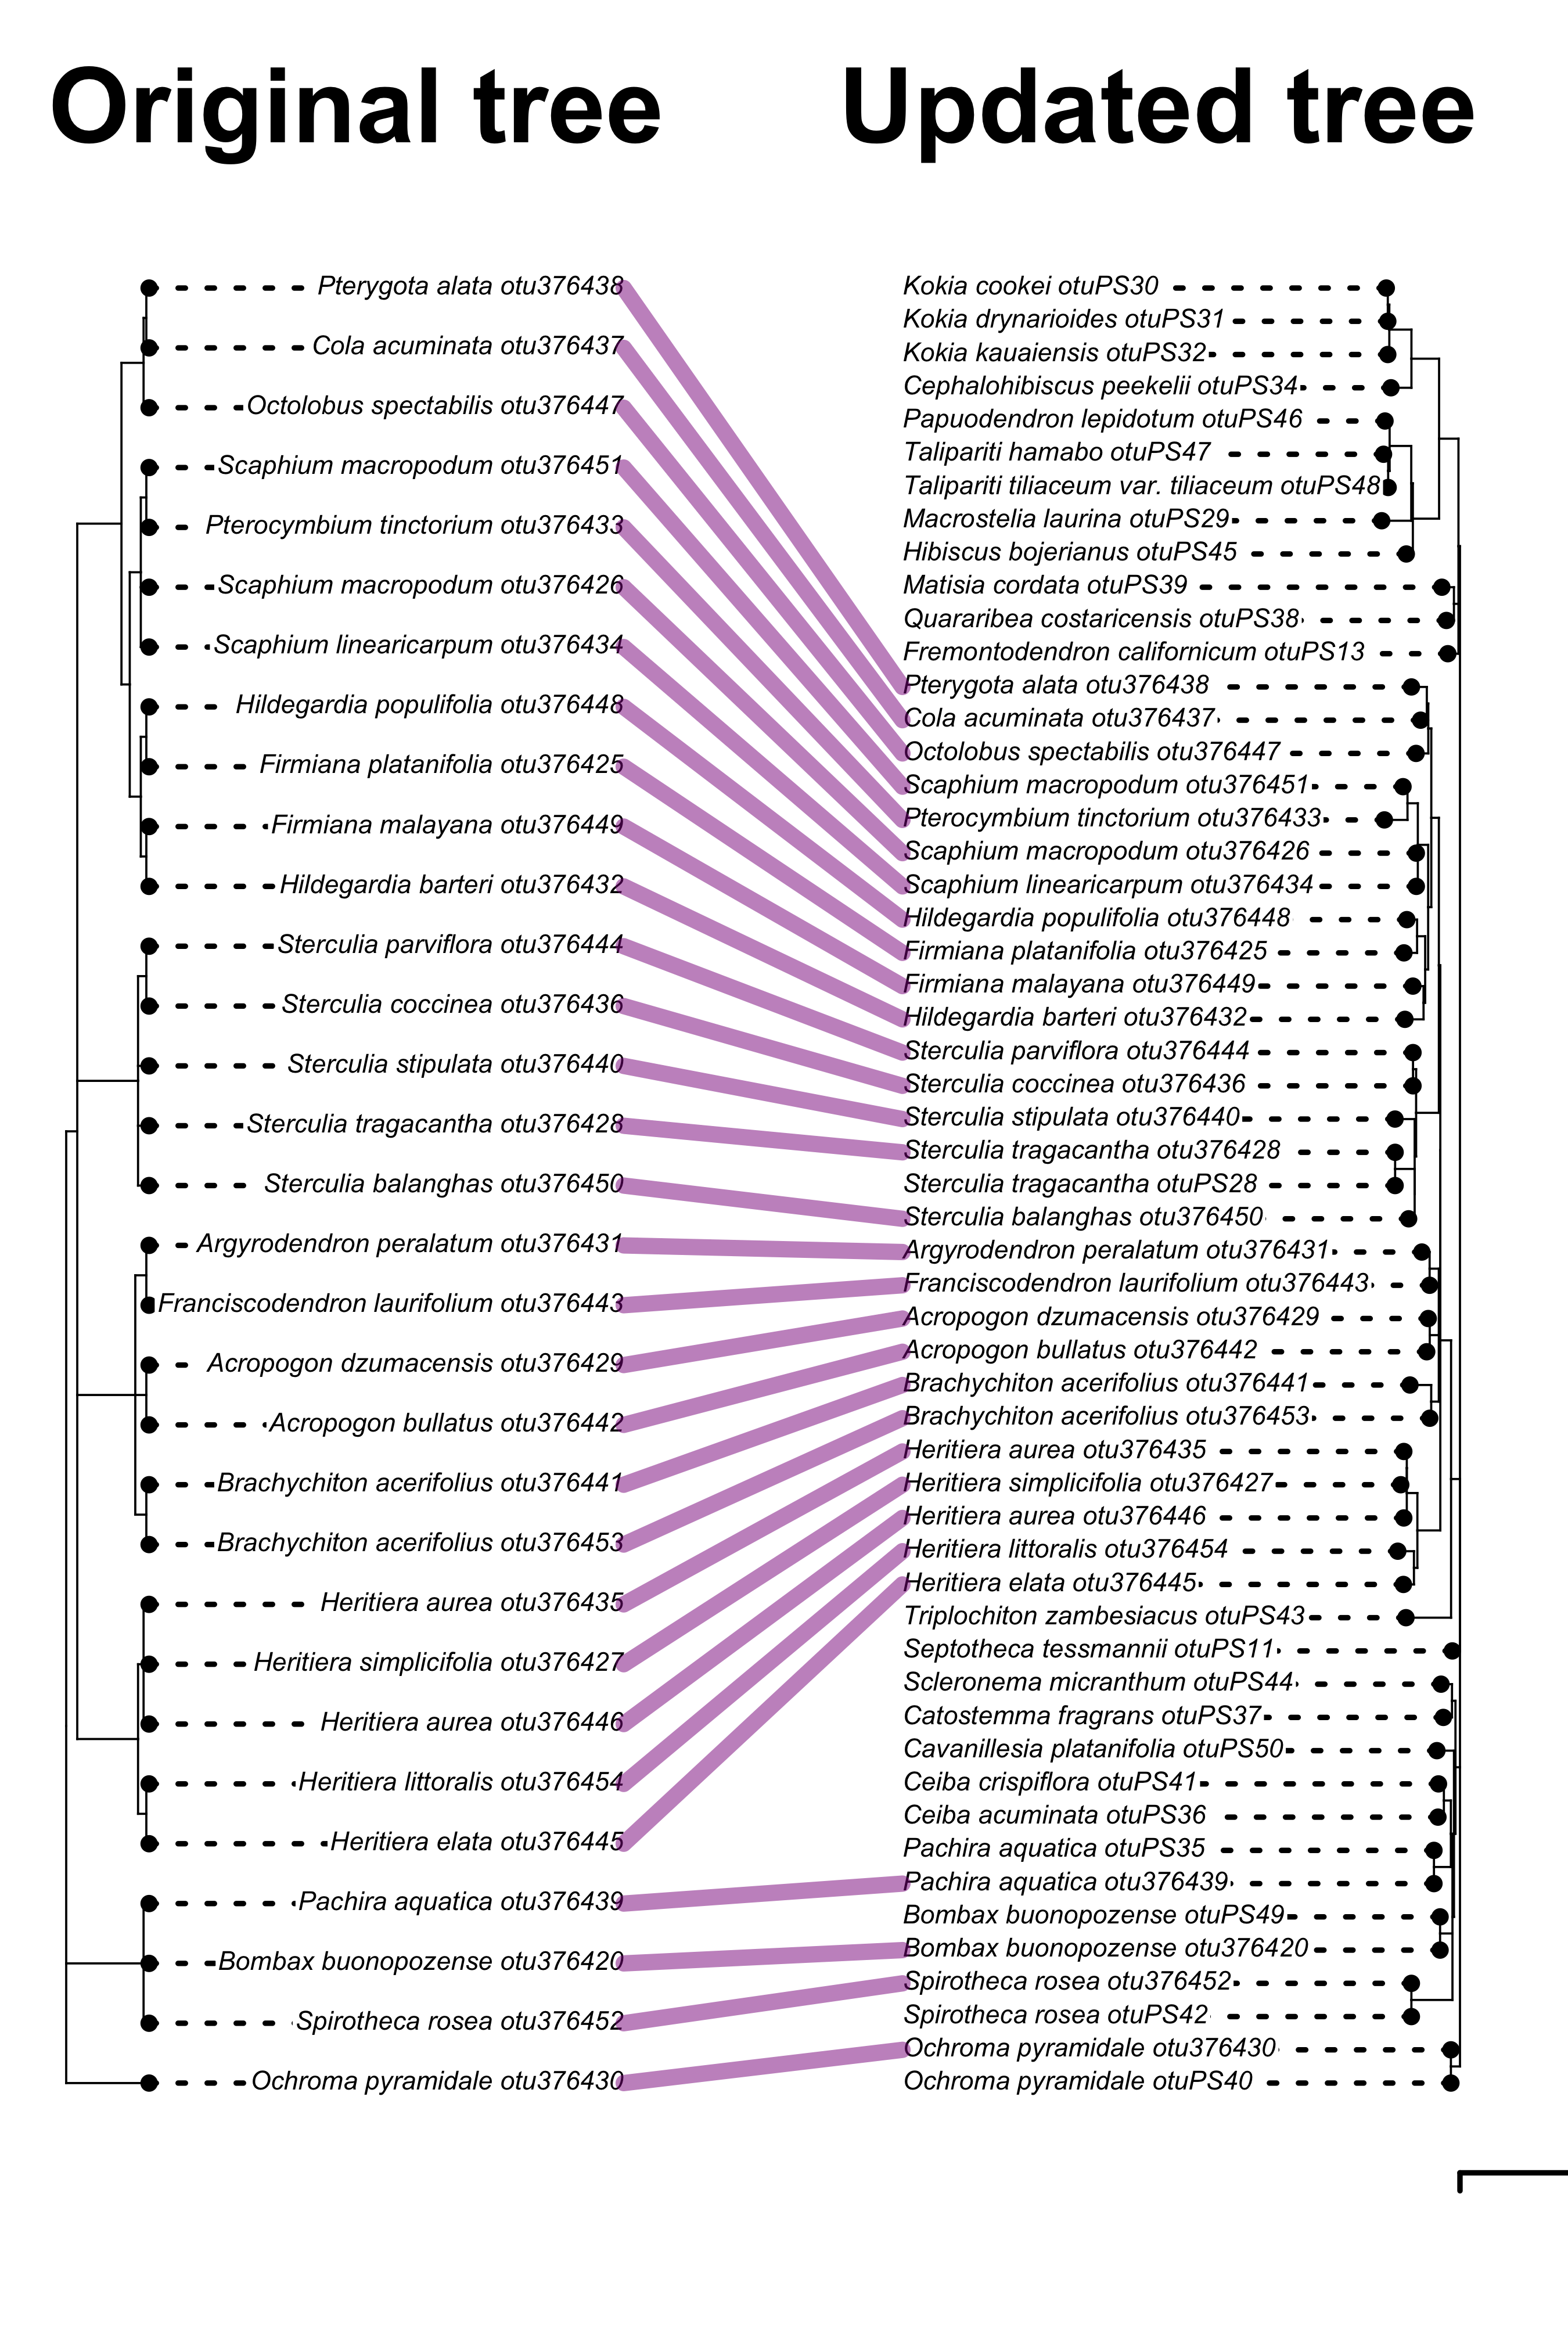
\includegraphics[width=0.85\linewidth]{docs/figs/cotree-plot2-1} 

}

\caption{Comparison of original tree and tree updated with Physcraper, family Malvaceae.}\label{fig:fig-2}
\end{figure}
\newpage

\hypertarget{discussion}{%
\section{Discussion}\label{discussion}}

Data repositories hold even more information than meets the eye.
Besides the actual data, they are rich sources of metadata that can be used for the advantage of biology and science in general.

Many pipelines are making use of DNA data repositories in different ways.
Most of them focus on efficient ways to mine the data -- getting the most homologs.
Some focus on accurate ways of mining the data -- getting real and clean homologs.
Others focus on refining the alignment.
Most focus on generating full trees \emph{de novo}, mainly for regions of the Tree of
Life that have no phylogenetic assessment yet in published studies, but also for
regions that have been already studied and that have phylogenetic data already.
However, expert phylogenetic knowledge is also an important source of data in public
and open repositories that is not being used to its full potential.

All these tools are key efforts for advancing towards reproducibility in phylogenetics,
a field that has relied on processes which are somewhat artisanal.
In here, we highlight the potential of taking advantage of this careful curation work in previous phylogenetic estimates. By taking sources of information available from data repositories and present a method to link data from different repositories, while leveraging on the knowledge and intuition of the expert
community to build up our phylogenetic knowledge, we can use not only data accumulated in
molecular data repositories, but phylogenetic knowledge accumulated in phylogenetic tree repositories.
While not generating full phylogenies \emph{de novo}, Physcraper is still capable of generating new phylogenetic knowledge.
It can also be combined with data from repositories other than molecular data. For example geographic locations (GBIF), fossils (PBDB), etc.

Physcraper has the potential to be applied for the advantage of the field to rapidly
place newly discovered species phylogenetically (Webb \emph{et al.} \protect\hyperlink{ref-webb2010biodiversity}{2010}),
obtain trees for ecophylogenetic studies (Helmus \& Ives \protect\hyperlink{ref-helmus2012phylogenetic}{2012}),
help to systematize molecular databases, i.e., curate taxonomic assignations (San Mauro \& Agorreta \protect\hyperlink{ref-san2010molecular}{2010}),
and rapidly generate custom species trees for downstream analyses (Stoltzfus \emph{et al.} \protect\hyperlink{ref-stoltzfus2013phylotastic}{2013}).

\hypertarget{acknowledgements}{%
\section{Acknowledgements}\label{acknowledgements}}

Research was supported by the grant ``Sustaining the Open Tree of Life'', National Science Foundation ABI No.~1759838, and ABI No.~1759846.
Compute time was provided by the Multi-Environment Research Computer for Exploration and Discovery (MERCED) cluster from the University of California, Merced (UCM), supported by the NSF Grant No.~ACI-1429783.

We thank members of the ``short bar'' Science and Engineering Building 1, UCM, joint lab paper discussion meeting for valuable comments on a first version of this manuscript.

\hypertarget{authors-contributions}{%
\section{Authors' Contributions}\label{authors-contributions}}

\hypertarget{data-avilability}{%
\section{Data Avilability}\label{data-avilability}}

\newpage

\hypertarget{references}{%
\section{References}\label{references}}

\newpage
\begin{center}
\textsc{References}
\end{center}

\hypertarget{refs}{}
\leavevmode\hypertarget{ref-altschul1990basic}{}%
Altschul, S.F., Gish, W., Miller, W., Myers, E.W. \& Lipman, D.J. (1990). Basic local alignment search tool. \emph{Journal of molecular biology}, \textbf{215}, 403--410.

\leavevmode\hypertarget{ref-altschul1997gapped}{}%
Altschul, S.F., Madden, T.L., Schäffer, A.A., Zhang, J., Zhang, Z., Miller, W. \& Lipman, D.J. (1997). Gapped blast and psi-blast: A new generation of protein database search programs. \emph{Nucleic acids research}, \textbf{25}, 3389--3402.

\leavevmode\hypertarget{ref-antonelli2017toward}{}%
Antonelli, A., Hettling, H., Condamine, F.L., Vos, K., Nilsson, R.H., Sanderson, M.J., Sauquet, H., Scharn, R., Silvestro, D., Töpel, M. \& others. (2017). Toward a self-updating platform for estimating rates of speciation and migration, ages, and relationships of taxa. \emph{Systematic Biology}, \textbf{66}, 152--166.

\leavevmode\hypertarget{ref-benson2000genbank}{}%
Benson, D.A., Karsch-Mizrachi, I., Lipman, D.J., Ostell, J., Rapp, B.A. \& Wheeler, D.L. (2000). GenBank. \emph{Nucleic acids research}, \textbf{28}, 15--18.

\leavevmode\hypertarget{ref-camacho2009blast}{}%
Camacho, C., George, C., Vahram, A., Ning, M., Jason, P., Kevin, B. \& Thomas, L. (2009). BLAST+: Architecture and applications. \emph{BMC bioinformatics}, \textbf{10}, 421.

\leavevmode\hypertarget{ref-cock2009biopython}{}%
Cock, P.J., Antao, T., Chang, J.T., Chapman, B.A., Cox, C.J., Dalke, A., Friedberg, I., Hamelryck, T., Kauff, F., Wilczynski, B. \& others. (2009). Biopython: Freely available python tools for computational molecular biology and bioinformatics. \emph{Bioinformatics}, \textbf{25}, 1422--1423.

\leavevmode\hypertarget{ref-drew2013lost}{}%
Drew, B.T., Gazis, R., Cabezas, P., Swithers, K.S., Deng, J., Rodriguez, R., Katz, L.A., Crandall, K.A., Hibbett, D.S. \& Soltis, D.E. (2013). Lost branches on the tree of life. \emph{PLoS biology}, \textbf{11}.

\leavevmode\hypertarget{ref-eaton2016misconceptions}{}%
Eaton, D.A.R., Spriggs, E.L., Park, B. \& Donoghue, M.J. (2016). Misconceptions on Missing Data in RAD-seq Phylogenetics with a Deep-scale Example from Flowering Plants. \emph{Systematic Biology}, \textbf{66}, 399--412. Retrieved from \url{https://doi.org/10.1093/sysbio/syw092}

\leavevmode\hypertarget{ref-edgar2004muscle}{}%
Edgar, R.C. (2004). MUSCLE: Multiple sequence alignment with high accuracy and high throughput. \emph{Nucleic acids research}, \textbf{32}, 1792--1797.

\leavevmode\hypertarget{ref-fragoso2017pilot}{}%
Fragoso-Martínez, I., Salazar, G.A., Martínez-Gordillo, M., Magallón, S., Sánchez-Reyes, L., Lemmon, E.M., Lemmon, A.R., Sazatornil, F. \& Mendoza, C.G. (2017). A pilot study applying the plant anchored hybrid enrichment method to new world sages (salvia subgenus calosphace; lamiaceae). \emph{Molecular Phylogenetics and Evolution}, \textbf{117}, 124--134.

\leavevmode\hypertarget{ref-helmus2012phylogenetic}{}%
Helmus, M.R. \& Ives, A.R. (2012). Phylogenetic diversity--area curves. \emph{Ecology}, \textbf{93}, S31--S43.

\leavevmode\hypertarget{ref-hinchliff2015synthesis}{}%
Hinchliff, C.E., Smith, S.A., Allman, J.F., Burleigh, J.G., Chaudhary, R., Coghill, L.M., Crandall, K.A., Deng, J., Drew, B.T., Gazis, R. \& others. (2015). Synthesis of phylogeny and taxonomy into a comprehensive tree of life. \emph{Proceedings of the National Academy of Sciences}, \textbf{112}, 12764--12769.

\leavevmode\hypertarget{ref-izquierdo-carrasco_pumper:_2014}{}%
Izquierdo-Carrasco, F., Cazes, J., Smith, S.A. \& Stamatakis, A. (2014). PUmPER: Phylogenies Updated Perpetually. \emph{Bioinformatics}, \textbf{30}, 1476--7. Retrieved February 1, 2014, from \url{http://bioinformatics.oxfordjournals.org/content/early/2014/01/28/bioinformatics.btu053}

\leavevmode\hypertarget{ref-magee2014dawn}{}%
Magee, A.F., May, M.R. \& Moore, B.R. (2014). The dawn of open access to phylogenetic data. \emph{PLoS One}, \textbf{9}.

\leavevmode\hypertarget{ref-mctavish2018bioessay}{}%
McTavish, E.J., Drew, B.T., Redelings, B. \& Cranston, K.A. (2017). How and Why to Build a Unified Tree of Life. \emph{BioEssays}, \textbf{39}. Retrieved April 10, 2018, from \url{https://onlinelibrary.wiley.com/doi/abs/10.1002/bies.201700114}

\leavevmode\hypertarget{ref-mctavish2015phylesystem}{}%
McTavish, E.J., Hinchliff, C.E., Allman, J.F., Brown, J.W., Cranston, K.A., Holder, M.T., Rees, J.A. \& Smith, S.A. (2015). Phylesystem: A git-based data store for community-curated phylogenetic estimates. \emph{Bioinformatics}, \textbf{31}, 2794--2800.

\leavevmode\hypertarget{ref-morrison2006multiple}{}%
Morrison, D.A. (2006). Multiple sequence alignment for phylogenetic purposes. \emph{Australian Systematic Botany}, \textbf{19}, 479--539.

\leavevmode\hypertarget{ref-opentreeoflife2019synth}{}%
OpenTreeOfLife, Redelings, B., Reyes, L.L.S., Cranston, K.A., Allman, J., Holder, M.T. \& McTavish, E.J. (2019). Open tree of life synthetic tree. Retrieved from \url{https://doi.org/10.5281/zenodo.3937742}

\leavevmode\hypertarget{ref-piel2009treebase}{}%
Piel, W., Chan, L., Dominus, M., Ruan, J., Vos, R. \& Tannen, V. (2009). Treebase v. 2: A database of phylogenetic knowledge. E-biosphere.

\leavevmode\hypertarget{ref-redelings2017supertree}{}%
Redelings, B.D. \& Holder, M.T. (2017). A supertree pipeline for summarizing phylogenetic and taxonomic information for millions of species. \emph{PeerJ}, \textbf{5}, e3058.

\leavevmode\hypertarget{ref-rees2017automated}{}%
Rees, J.A. \& Cranston, K. (2017). Automated assembly of a reference taxonomy for phylogenetic data synthesis. \emph{Biodiversity Data Journal}.

\leavevmode\hypertarget{ref-sanderson2008phylota}{}%
Sanderson, M.J., Boss, D., Chen, D., Cranston, K.A. \& Wehe, A. (2008). The PhyLoTA Browser: Processing GenBank for Molecular Phylogenetics Research. \emph{Systematic Biology}, \textbf{57}, 335--346.

\leavevmode\hypertarget{ref-san2010molecular}{}%
San Mauro, D. \& Agorreta, A. (2010). Molecular systematics: A synthesis of the common methods and the state of knowledge. \emph{Cellular \& Molecular Biology Letters}, \textbf{15}, 311.

\leavevmode\hypertarget{ref-smith2009mega}{}%
Smith, S.A., Beaulieu, J.M. \& Donoghue, M.J. (2009). Mega-phylogeny approach for comparative biology: An alternative to supertree and supermatrix approaches. \emph{BMC evolutionary biology}, \textbf{9}, 37.

\leavevmode\hypertarget{ref-song2012resolving}{}%
Song, S., Liu, L., Edwards, S.V. \& Wu, S. (2012). Resolving conflict in eutherian mammal phylogeny using phylogenomics and the multispecies coalescent model. \emph{Proceedings of the National Academy of Sciences}, \textbf{109}, 14942--14947.

\leavevmode\hypertarget{ref-stamatakis2014raxml}{}%
Stamatakis, A. (2014). RAxML version 8: A tool for phylogenetic analysis and post-analysis of large phylogenies. \emph{Bioinformatics}, \textbf{30}, 1312--1313.

\leavevmode\hypertarget{ref-stoltzfus2013phylotastic}{}%
Stoltzfus, A., Lapp, H., Matasci, N., Deus, H., Sidlauskas, B., Zmasek, C.M., Vaidya, G., Pontelli, E., Cranston, K., Vos, R. \& others. (2013). Phylotastic! Making tree-of-life knowledge accessible, reusable and convenient. \emph{BMC bioinformatics}, \textbf{14}, 158.

\leavevmode\hypertarget{ref-sukumaran2010dendropy}{}%
Sukumaran, J. \& Holder, M.T. (2010). DendroPy: A python library for phylogenetic computing. \emph{Bioinformatics}, \textbf{26}, 1569--1571.

\leavevmode\hypertarget{ref-vos2012nexml}{}%
Vos, R.A., Balhoff, J.P., Caravas, J.A., Holder, M.T., Lapp, H., Maddison, W.P., Midford, P.E., Priyam, A., Sukumaran, J., Xia, X. \& others. (2012). NeXML: Rich, extensible, and verifiable representation of comparative data and metadata. \emph{Systematic biology}, \textbf{61}, 675--689.

\leavevmode\hypertarget{ref-webb2010biodiversity}{}%
Webb, C.O., Slik, J.F. \& Triono, T. (2010). Biodiversity inventory and informatics in southeast asia. \emph{Biodiversity and Conservation}, \textbf{19}, 955--972.

\leavevmode\hypertarget{ref-wheeler2000database}{}%
Wheeler, D.L., Chappey, C., Lash, A.E., Leipe, D.D., Madden, T.L., Schuler, G.D., Tatusova, T.A. \& Rapp, B.A. (2000). Database resources of the national center for biotechnology information. \emph{Nucleic acids research}, \textbf{28}, 10--14.

\end{document}
